%\chapter{Vorlesung}
\chapter{(a,b)-Suchbäume}
Blattorientierte Speicherung der Elemente\\
Innere Knoten haben mindestens a und höchstens b Kinder und tragen entsprechende Schlüsselwerte, um die Suche zu leiten.
\paragraph{Beispiel:}
$ $
\begin{figure}[H]
\centering
\begin{subfigure}[H]{0.6\linewidth}
	\centering
	\captionabove*{2-5 Bäume}
	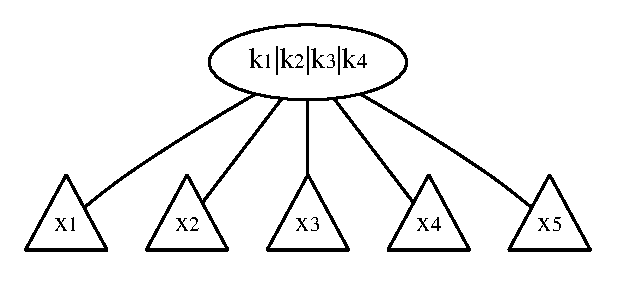
\includegraphics[width=0.8\linewidth]{12/Grafik/graph1}
	\caption{$x_1\leq k_1<x_2\leq k_2<x_3\leq K_3<x_4\leq k_4<x_5$}
	\label{fig:graph1}
\end{subfigure}
\begin{subfigure}[H]{0.3\linewidth}
	\centering
	\captionabove*{Knotengrad$=2$}
	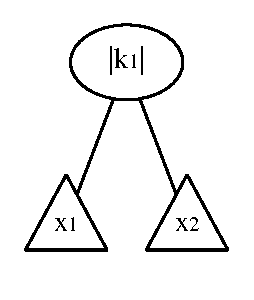
\includegraphics[width=0.7\linewidth]{12/Grafik/graph2}
	\caption{$x_1\leq k_1<x_2$}
	\label{fig:graph2}
\end{subfigure}
\end{figure}

\[h\hat{=}\text{Tiefe}\Rightarrow ~~ a^h\leq n \leq b^h ~\Rightarrow ~ \log_b n \leq h \leq \log_a n\]
\begin{figure}[h]
\centering
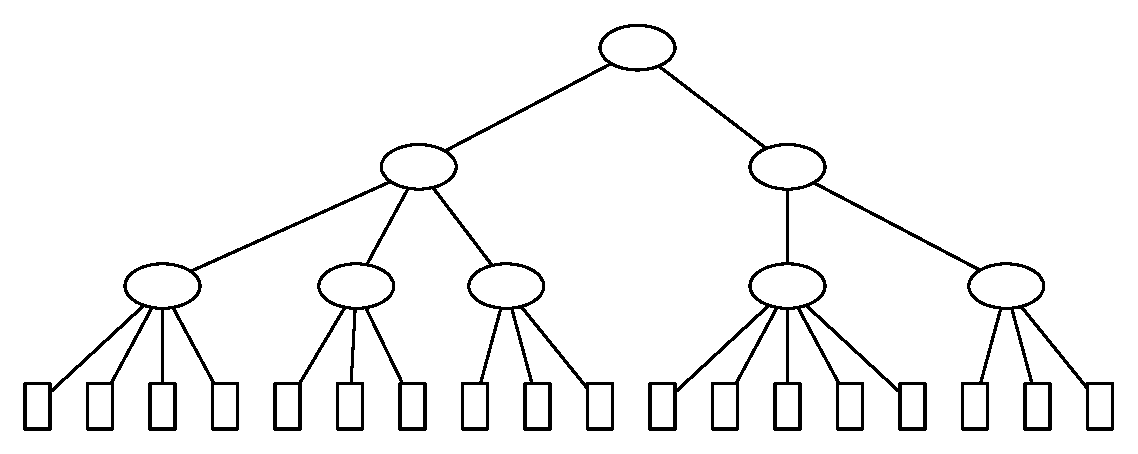
\includegraphics[width=\linewidth]{12/Grafik/graph3}
\caption{Einfügen und Löschen in einem 2-5 Baum}
\label{fig:graph3}
\end{figure}

\section{Aufspaltung bei Einfügen}
$ $
\begin{figure}[H]
	\centering
	\begin{subfigure}[H]{0.4\linewidth}
		\centering
		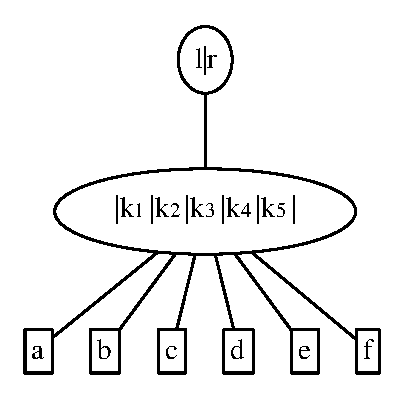
\includegraphics[width=\linewidth]{12/Grafik/graph4}
		\caption{$a<b<c<d<e<f$}
		\label{fig:graph4}
	\end{subfigure}
	{\Huge $\Rightarrow$}
	\begin{subfigure}[H]{0.4\linewidth}
		\centering
		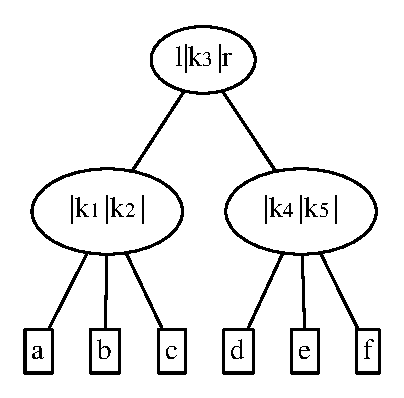
\includegraphics[width=\linewidth]{12/Grafik/graph5}
		\caption{$a<b<c<d<e<f$}
		\label{fig:graph5}
	\end{subfigure}
\end{figure}
\section{Verschmelzen von Knoten beim Löschen}
$ $
\begin{figure}[H]
	\centering
	\begin{subfigure}[H]{0.4\linewidth}
		\centering
		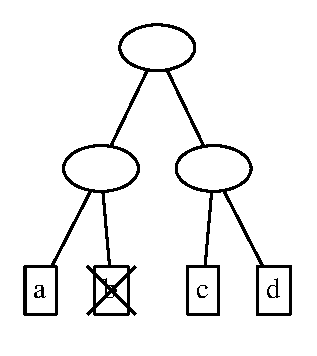
\includegraphics[width=\linewidth]{12/Grafik/graph6}
		\caption{$b$ wird gelöscht}
		\label{fig:graph6}
	\end{subfigure}
	{\Huge $\Rightarrow$}
	\begin{subfigure}[H]{0.4\linewidth}
		\centering
		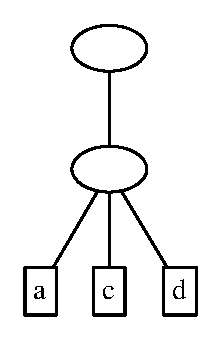
\includegraphics[width=0.675\linewidth]{12/Grafik/graph7}
		\caption{Baum ohne $b$}
		\label{fig:graph7}
	\end{subfigure}
\end{figure}
Aufspalte- und Verschmelze-Operationen können sich von der Blattebene bis zur Wurzel kaskadenartig fortpflanzen. Sie bleiben aber auf den Suchpfad begrenzt.\\
$\Rightarrow$ Umbaukosten sind beschränkt durch die Baumtiefe $=O(\log n)$
\chapter{Amortisierte Analyse}
\paragraph{Beispiel: Binärzähler}
	\begin{tabular}{lr}
		$000$& \\
		$001$&$\text{Kosten}(1)=1$\\
		$010$&$=2$\\
		$011$&$=1$\\
		$100$&$=3$\\
		$101$&$=1$\\
		$110$&$=2$\\
		$111$&$=1$\\
		 &$\overline{11}$
	\end{tabular}
	Kosten der Inkrement-Operation $\hat{=}$ Zahl der Bit-Flips\\
	Naive Analyse $2^k=n$
	\[1\cdot\frac{n}{2}+2\cdot\frac{n}{4}+3\cdot\frac{n}{8}+\ldots+k\cdot\frac{n}{2^k}=\frac{n}{2}\sum_{i=1}^{k}i(\frac{1}{2})^{i-1}=2^{k+1}-k-2=2n-k-2 \]
Von $0$ bis $n$ im Binärsystem zu zählen kostet  $\leq 2n$ Bit-Flips
\paragraph{Sprechweise:} amortisierte Kosten einer Inkrement-Operation sind $2$\\
Folge von n-Ops kostet $2n$
\section{Bankkonto-Methode}
\[\text{Konto}(i+1)=\text{Konto}(i)-\text{Kosten}(i)+\text{Einzahlung}(i) \]
\[\sum_{i=1}^{n}\text{Kosten}(i)=\text{tatsächliche Gesamtkosten} = \sum_{i=1}^{n}(\text{Einzahlung}(i)+\text{Konto}(i-\text{Konto}(i+1))\]
\[=\sum_{i=1}^{n}\text{Einzahlung}(i)+\text{Konto}(1)-\text{Konto}(n+1) \]
	\begin{tabular}{lr}
		$000$& \\
		$001_\text{\euro}$&$\text{Kosten}(1)=1$\\
		$01_\text{€}0$&$=2$\\
		$01_\text{€}1_\text{€}$&$=1$\\
		$1_\text{€}00$&$=3$\\
		$1_\text{€}01_\text{€}$&$=1$\\
		$1_\text{€}1_\text{€}0$&$=2$\\
		$1_\text{€}1_\text{€}1_\text{€}$&$=1$\\
		&$\overline{11}$
	\end{tabular}
	\pagebreak
	\subsection{Kontoführungsschema: für Binärzähler}
	1€ pro 1 in der Binärdarstellung\\
	Jeder Übergang $1_\text{€}\rightarrow0$ kann dann mit dem entsprechenden Euro Betrag auf dieser 1 bezahlt werden.\\
	Es gibt pro Inkrement Operation nur einen $0\rightarrow1$ Übergang\\
	2€ Einzahlung für jede Inc-Operation reichen aus um:
	\begin{enumerate}
		\item diesen $0\rightarrow1$ Übergang zu bezahlen
		\item die neu entstandene $1_\text{€}$ mit einem Euro zu besparen.
	\end{enumerate}
	\[\text{GK} = 2(2^k-1)+0\footnote{Zählerstand(000)}-k\footnote{Zählerstand($\overbrace{111\ldots1}^k$)}=2n-k-2\]